\documentclass[11pt, a4paper]{article}

\usepackage[T1]{fontenc}
\usepackage[utf8]{inputenc}
\usepackage[provide=*,polish]{babel}
\usepackage{geometry}
\usepackage{xcolor}
\usepackage{titlesec}
\usepackage{enumitem}
\usepackage{tabularx}
\usepackage{booktabs}
\usepackage{fancyhdr}
\usepackage{mdframed}
\usepackage{tikz}
\usepackage{pgf}
\usepackage{hyperref}
\usepackage{parskip}
\usepackage{array}
\usepackage{multirow}
\usepackage{tcolorbox}
\tcbuselibrary{skins, breakable}
\usetikzlibrary{shapes.geometric, arrows.meta, positioning, fit, backgrounds, calc}

\geometry{
  top=2.2cm, bottom=2.5cm,
  left=2.4cm, right=2.4cm,
  headheight=14pt
}

\definecolor{primary}{HTML}{1A1A2E}
\definecolor{accent}{HTML}{E94560}
\definecolor{accentsoft}{HTML}{FF6B6B}
\definecolor{secondary}{HTML}{0F3460}
\definecolor{lightbg}{HTML}{F4F4F8}
\definecolor{mutedgray}{HTML}{8A8A9A}
\definecolor{done}{HTML}{2ECC71}
\definecolor{todo}{HTML}{F39C12}
\definecolor{wireframe}{HTML}{BDC3C7}
\definecolor{wirebg}{HTML}{F8F9FA}

\titleformat{\section}
  {\color{primary}\Large\bfseries}
  {}
  {0em}
  {\colorbox{accent}{\makebox[0.5cm][c]{\color{white}\thesection}}\quad}
  [\vspace{2pt}\color{accent}\hrule height 0.8pt\vspace{4pt}]

\titleformat{\subsection}
  {\color{secondary}\normalsize\bfseries}
  {\thesubsection\enspace}
  {0em}
  {}

\titlespacing*{\section}{0pt}{18pt}{8pt}
\titlespacing*{\subsection}{0pt}{10pt}{4pt}

\pagestyle{fancy}
\fancyhf{}
\renewcommand{\headrulewidth}{0pt}
\fancyhead[L]{%
  \small\color{mutedgray}\textbf{SalFit} \textbar\ Dokumentacja Sprintu 2}
\fancyhead[R]{%
  \small\color{mutedgray}Inżynieria Oprogramowania · 2025/2026}
\fancyfoot[C]{\small\color{mutedgray}\thepage}

\tcbset{
  donebox/.style={
    colback=done!8, colframe=done!60,
    boxrule=0.8pt, arc=4pt,
    left=8pt, right=8pt, top=6pt, bottom=6pt,
    fonttitle=\bfseries\small\color{done!80!black},
    title={{\small\textbf{DONE}} ~---~ zrealizowane}
  },
  epicbox/.style={
    colback=secondary!5, colframe=secondary!30,
    boxrule=0.8pt, arc=4pt,
    left=8pt, right=8pt, top=6pt, bottom=6pt,
    fonttitle=\bfseries\small\color{secondary},
  },
  infobox/.style={
    colback=lightbg, colframe=accent!40,
    boxrule=0.8pt, arc=4pt,
    left=8pt, right=8pt, top=6pt, bottom=6pt,
  },
  todobox/.style={
    colback=todo!8, colframe=todo!60,
    boxrule=0.8pt, arc=4pt,
    left=8pt, right=8pt, top=6pt, bottom=6pt,
    fonttitle=\bfseries\small\color{todo!80!black},
    title={{\small\textbf{TODO}} ~---~ zaplanowane}
  }
}

\newcommand{\tag}[2][accent]{%
  \colorbox{#1!15}{\small\color{#1!80!black}\textbf{#2}}%
}
\newcommand{\actor}[1]{\textit{\color{secondary}#1}}

\begin{document}

% ═══════════════════════════════════════════════════════════════════════════════
%  COVER
% ═══════════════════════════════════════════════════════════════════════════════
\thispagestyle{empty}

\begin{tikzpicture}[remember picture, overlay]
  \fill[primary] (current page.north west) rectangle
    ([yshift=-6cm] current page.north east);
  \fill[accent] ([yshift=-6cm] current page.north west) rectangle
    ([yshift=-6.4cm] current page.north east);
\end{tikzpicture}

\vspace*{0.6cm}
{\color{white}\fontsize{36}{42}\selectfont\bfseries SalFit}\\[6pt]
{\color{accent!80}\large System zarządzania organizacją sal fitness}\\[4pt]
{\color{white!70}\small Dokumentacja Sprintu 2 \textbar\ Inżynieria Oprogramowania · 2025/2026}

\vspace{3.2cm}

\begin{tcolorbox}[infobox, title={}]
\begin{tabularx}{\linewidth}{@{}lX@{}}
  \textbf{Lider projektu}   & Konrad Mytnik (\texttt{SliceOf314159}) \\[3pt]
  \textbf{Członek zespołu}  & Bartek Małecki (\texttt{malkiinho}) \\[3pt]
  \textbf{Repozytorium}     & \href{https://github.com/SliceOf314159/salFit}{\texttt{github.com/SliceOf314159/salFit}} \\[3pt]
  \textbf{Tablica Kanban}   & \href{https://github.com/users/SliceOf314159/projects/1}{\texttt{github.com/users/SliceOf314159/projects/1}} \\
\end{tabularx}
\end{tcolorbox}

\newpage

% ═══════════════════════════════════════════════════════════════════════════════
%  1. WIZJA SYSTEMU
% ═══════════════════════════════════════════════════════════════════════════════
\section{Wizja systemu}

System \textbf{SalFit} służy do kompleksowego zarządzania organizacją siłowni i sal fitness.
Umożliwia administratorom dodawanie i edytowanie profili trenerów, zarządzanie statusem sal
(\emph{dostępna}, \emph{zajęta}, \emph{w remoncie}), tworzenie grafiku zajęć oraz przypisywanie
trenerów do konkretnych sal i terminów. System pozwala również na rejestrację członków,
śledzenie ich karnetów oraz generowanie podstawowych raportów obłożenia.

Celem systemu jest usprawnienie codziennej obsługi obiektu i zastąpienie ręcznego planowania
jednym centralnym narzędziem.

\medskip
\tag[secondary]{Java} \tag[secondary]{JavaFX} \tag[secondary]{JSON/CSV} \tag[secondary]{Desktop}

\bigskip
Projekt realizowany jest w języku \textbf{Java} z interfejsem graficznym opartym na
\textbf{JavaFX}. Dane przechowywane są lokalnie w pliku (mock bazy danych) — bez zewnętrznego
silnika bazodanowego.

% ═══════════════════════════════════════════════════════════════════════════════
%  2. ZAKRES USŁUG
% ═══════════════════════════════════════════════════════════════════════════════
\section{Zakres usług}

\subsection{Co zostanie zrealizowane}

\begin{itemize}[leftmargin=*, itemsep=2pt]
  \item \textbf{Zarządzanie trenerami} — dodawanie, edycja, usuwanie, przeglądanie listy
  \item \textbf{Zarządzanie salami} — dodawanie sal, zmiana statusu
  \item \textbf{Grafik zajęć} — przypisywanie trenerów do sal i terminów, podgląd tygodniowy
  \item \textbf{Zarządzanie członkami} — rejestracja, przeglądanie, edycja danych
  \item \textbf{Karnety} — przypisywanie do członków, śledzenie dat ważności
  \item \textbf{Moduł raportów} — obłożenie sal, aktywność trenerów, status karnetów
  \item \textbf{Persystencja danych} — zapis/odczyt z pliku JSON/CSV
  \item \textbf{Interfejs graficzny JavaFX} z nawigacją między modułami
\end{itemize}

\subsection{Co NIE zostanie zrealizowane}

\begin{itemize}[leftmargin=*, itemsep=2pt, label=\color{accent}$\times$]
  \item Integracja z zewnętrzną bazą danych (MySQL, PostgreSQL)
  \item System płatności i fakturowania
  \item Aplikacja mobilna
  \item Powiadomienia e-mail / SMS
  \item Uwierzytelnianie i system ról użytkowników
  \item Dostęp wielostanowiskowy / sieciowy
\end{itemize}

% ═══════════════════════════════════════════════════════════════════════════════
%  3. ARCHITEKTURA LOGICZNA
% ═══════════════════════════════════════════════════════════════════════════════
\section{Architektura logiczna}

System SalFit oparty jest na \textbf{trójwarstwowej architekturze} dostosowanej do środowiska
desktopowego JavaFX z lokalnym plikiem jako źródłem danych.

\bigskip

% Architecture diagram
\begin{center}
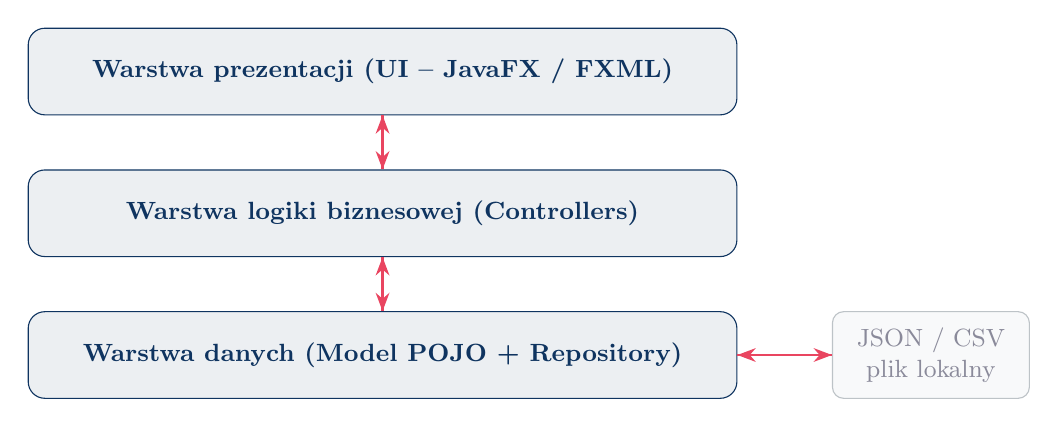
\begin{tikzpicture}[
  layer/.style={
    draw=secondary, fill=secondary!8, rounded corners=6pt,
    minimum width=9cm, minimum height=1.1cm,
    font=\bfseries\small\color{secondary}
  },
  arrow/.style={-Stealth, thick, color=accent}
]
  \node[layer] (ui)   at (0, 0)    {Warstwa prezentacji (UI -- JavaFX / FXML)};
  \node[layer] (biz)  at (0,-1.8)  {Warstwa logiki biznesowej (Controllers)};
  \node[layer] (data) at (0,-3.6)  {Warstwa danych (Model POJO + Repository)};

  \node[draw=wireframe, fill=wirebg, rounded corners=4pt,
        right=1.2cm of data, minimum width=2.5cm, minimum height=1.1cm,
        font=\small\color{mutedgray}, align=center] (file) {JSON / CSV\\plik lokalny};

  \draw[arrow] (ui) -- (biz);
  \draw[arrow] (biz) -- (ui);
  \draw[arrow] (biz) -- (data);
  \draw[arrow] (data) -- (biz);
  \draw[arrow] (data) -- (file);
  \draw[arrow] (file) -- (data);
\end{tikzpicture}
\end{center}

\bigskip

\subsection{Warstwa prezentacji (UI)}

Zbudowana w JavaFX z użyciem plików FXML. Każdy moduł posiada własny widok i kontroler.

\medskip
\begin{tabularx}{\linewidth}{@{}>{\ttfamily\small}lX@{}}
  \toprule
  \normalfont\textbf{Plik} & \textbf{Opis} \\
  \midrule
  MainView.fxml    & Główne okno, nawigacja \\
  TrenerView.fxml  & Zarządzanie trenerami \\
  SalaView.fxml    & Zarządzanie salami \\
  GrafikView.fxml  & Grafik zajęć \\
  CzlonekView.fxml & Zarządzanie członkami \\
  RaportView.fxml  & Moduł raportów \\
  \bottomrule
\end{tabularx}

\subsection{Warstwa logiki biznesowej (Controllers)}

Kontrolery JavaFX obsługują zdarzenia użytkownika i komunikują się z warstwą danych przez
klasy Repository. Nie zawierają logiki zapisu/odczytu plików.

\subsection{Warstwa danych (Model + Repository)}

Klasy POJO (\texttt{Trener}, \texttt{Sala}, \texttt{Karnet}, \texttt{Członek}) reprezentują
encje systemu. Klasy Repository odpowiadają za serializację/deserializację danych do/z pliku.
Dane przechowywane są w \newline
\texttt{src/main/resources/data/}.

% ═══════════════════════════════════════════════════════════════════════════════
%  4. GŁÓWNE FUNKCJE I EPIKI — USE CASE
% ═══════════════════════════════════════════════════════════════════════════════
\newpage
\section{Główne funkcje i epiki}

Poniżej przedstawiono historyjki użytkownika pogrupowane w epiki dla obu aktorów systemu: \actor{Administrator} oraz \actor{Trener}.

% ── Epiki ─────────────────────────────────────────────────────────────────────

\begin{tcolorbox}[epicbox, title={Epik 1 — Zarządzanie trenerami}]
\begin{itemize}[leftmargin=*, itemsep=2pt, label=\color{secondary}$\triangleright$]
  \item \actor{Administrator}: dodanie nowego trenera (imię, nazwisko, specjalizacja)
  \item \actor{Administrator}: edycja danych istniejącego trenera
  \item \actor{Administrator}: usunięcie trenera z systemu
  \item \actor{Administrator}: przeglądanie listy wszystkich trenerów
  \item \actor{Trener}: przeglądanie własnego profilu i specjalizacji
\end{itemize}
\end{tcolorbox}

\medskip

\begin{tcolorbox}[epicbox, title={Epik 2 — Zarządzanie salami}]
\begin{itemize}[leftmargin=*, itemsep=2pt, label=\color{secondary}$\triangleright$]
  \item \actor{Administrator}: dodanie nowej sali i określenie jej pojemności
  \item \actor{Administrator}: zmiana statusu sali (dostępna / zajęta / w remoncie)
  \item \actor{Administrator}: przeglądanie listy sal z aktualnym statusem
  \item \actor{Trener}: sprawdzenie statusu sali przypisanej do swoich zajęć
\end{itemize}
\end{tcolorbox}

\medskip

\begin{tcolorbox}[epicbox, title={Epik 3 — Grafik zajęć}]
\begin{itemize}[leftmargin=*, itemsep=2pt, label=\color{secondary}$\triangleright$]
  \item \actor{Administrator}: przypisanie trenera do sali w określonym terminie
  \item \actor{Administrator}: przeglądanie grafiku zajęć w układzie tygodniowym
  \item \actor{Administrator}: usunięcie lub zmiana przypisania trenera do zajęć
  \item \actor{Trener}: przeglądanie własnego grafiku zajęć (tygodniowy widok)
  \item \actor{Trener}: sprawdzenie przypisania do konkretnej sali i terminu
\end{itemize}
\end{tcolorbox}

\medskip

\begin{tcolorbox}[epicbox, title={Epik 4 — Zarządzanie członkami i karnetami}]
\begin{itemize}[leftmargin=*, itemsep=2pt, label=\color{secondary}$\triangleright$]
  \item \actor{Administrator}: rejestracja nowego członka klubu
  \item \actor{Administrator}: przypisanie karnetu do członka z datą ważności
  \item \actor{Administrator}: przeglądanie listy członków i statusu ich karnetów
  \item \actor{Administrator}: podgląd karnetów wygasających w ciągu 30 dni
  \item \actor{Trener}: przeglądanie listy uczestników przypisanych do swoich zajęć
\end{itemize}
\end{tcolorbox}

\medskip

\begin{tcolorbox}[epicbox, title={Epik 5 — Moduł raportów}]
\begin{itemize}[leftmargin=*, itemsep=2pt, label=\color{secondary}$\triangleright$]
  \item \actor{Administrator}: raport obłożenia sal w danym tygodniu
  \item \actor{Administrator}: raport aktywności trenerów (liczba zajęć)
  \item \actor{Administrator}: raport karnetów — aktywne, wygasłe, wygasające
  \item \actor{Administrator}: eksport raportu do pliku TXT lub CSV
  \item \actor{Trener}: przeglądanie raportu własnej aktywności (liczba przeprowadzonych zajęć)
\end{itemize}
\end{tcolorbox}

% ═══════════════════════════════════════════════════════════════════════════════
%  6. PODSUMOWANIE SPRINTU 2
% ═══════════════════════════════════════════════════════════════════════════════
\newpage
\section{Podsumowanie sprintu 2}

\begin{tcolorbox}[donebox]
\textbf{Konrad Mytnik}
\begin{itemize}[leftmargin=*, itemsep=3pt, label=\color{done}$\checkmark$]
  \item Utworzenie repozytorium GitHub (\texttt{salFit})
  \item Konfiguracja repozytorium — \texttt{.gitignore}, struktura katalogów
  \item Uzupełnienie \texttt{README}: skład zespołu, temat projektu, wizja systemu
  \item Opracowanie dokumentacji Sprint 2 (niniejszy dokument)
\end{itemize}

\medskip
\textbf{Bartek Małecki}
\begin{itemize}[leftmargin=*, itemsep=3pt, label=\color{done}$\checkmark$]
  \item Udział w tworzeniu tablicy Kanban w GitHub Projects
  \item Dodanie zadań do tablicy projektowej (kolumny TODO / DONE)
\end{itemize}

\medskip
\textbf{Wspólnie — Konrad Mytnik \& Bartek Małecki}
\begin{itemize}[leftmargin=*, itemsep=3pt, label=\color{done}$\checkmark$]
  \item Zdefiniowanie wizji systemu i zakresu projektu
  \item Opracowanie architektury trójwarstwowej (prezentacja / logika / dane)
  \item Sformułowanie epików i historyjek użytkownika (w tym dla aktora \actor{Trener})
  \item Konfiguracja i uruchomienie tablicy Kanban w GitHub Projects
  \item Przygotowanie makiet lo-fi interfejsu użytkownika
  \item Opracowanie diagramu aktywności
\end{itemize}
\end{tcolorbox}

\bigskip

\begin{tcolorbox}[todobox]
\textbf{Konrad Mytnik \& Bartek Małecki}
\begin{itemize}[leftmargin=*, itemsep=3pt, label=\color{todo}$\triangleright$]
  \item Przygotowanie raportu z badań interfejsu użytkownika
  \item Opracowanie diagramu klas (strona backendowa)
\end{itemize}
\end{tcolorbox}

\bigskip

\begin{tcolorbox}[infobox]
\small
\textbf{Linki do projektu:}\\[4pt]
Repozytorium GitHub: \url{https://github.com/SliceOf314159/salFit}\\
Tablica projektowa: \url{https://github.com/users/SliceOf314159/projects/1}
\end{tcolorbox}

\end{document}